This is the last day! Most of the regular/short paper presentation happen today.

\subsection{Short paper: Link and Graph Mining}

\subsubsection{LATTE: Application Oriented Social Network Embedding}
\ddef{Network embedding}{Map nodes in a network into a low-dimensional space}

\begin{figure}[ht!]
    \centering
    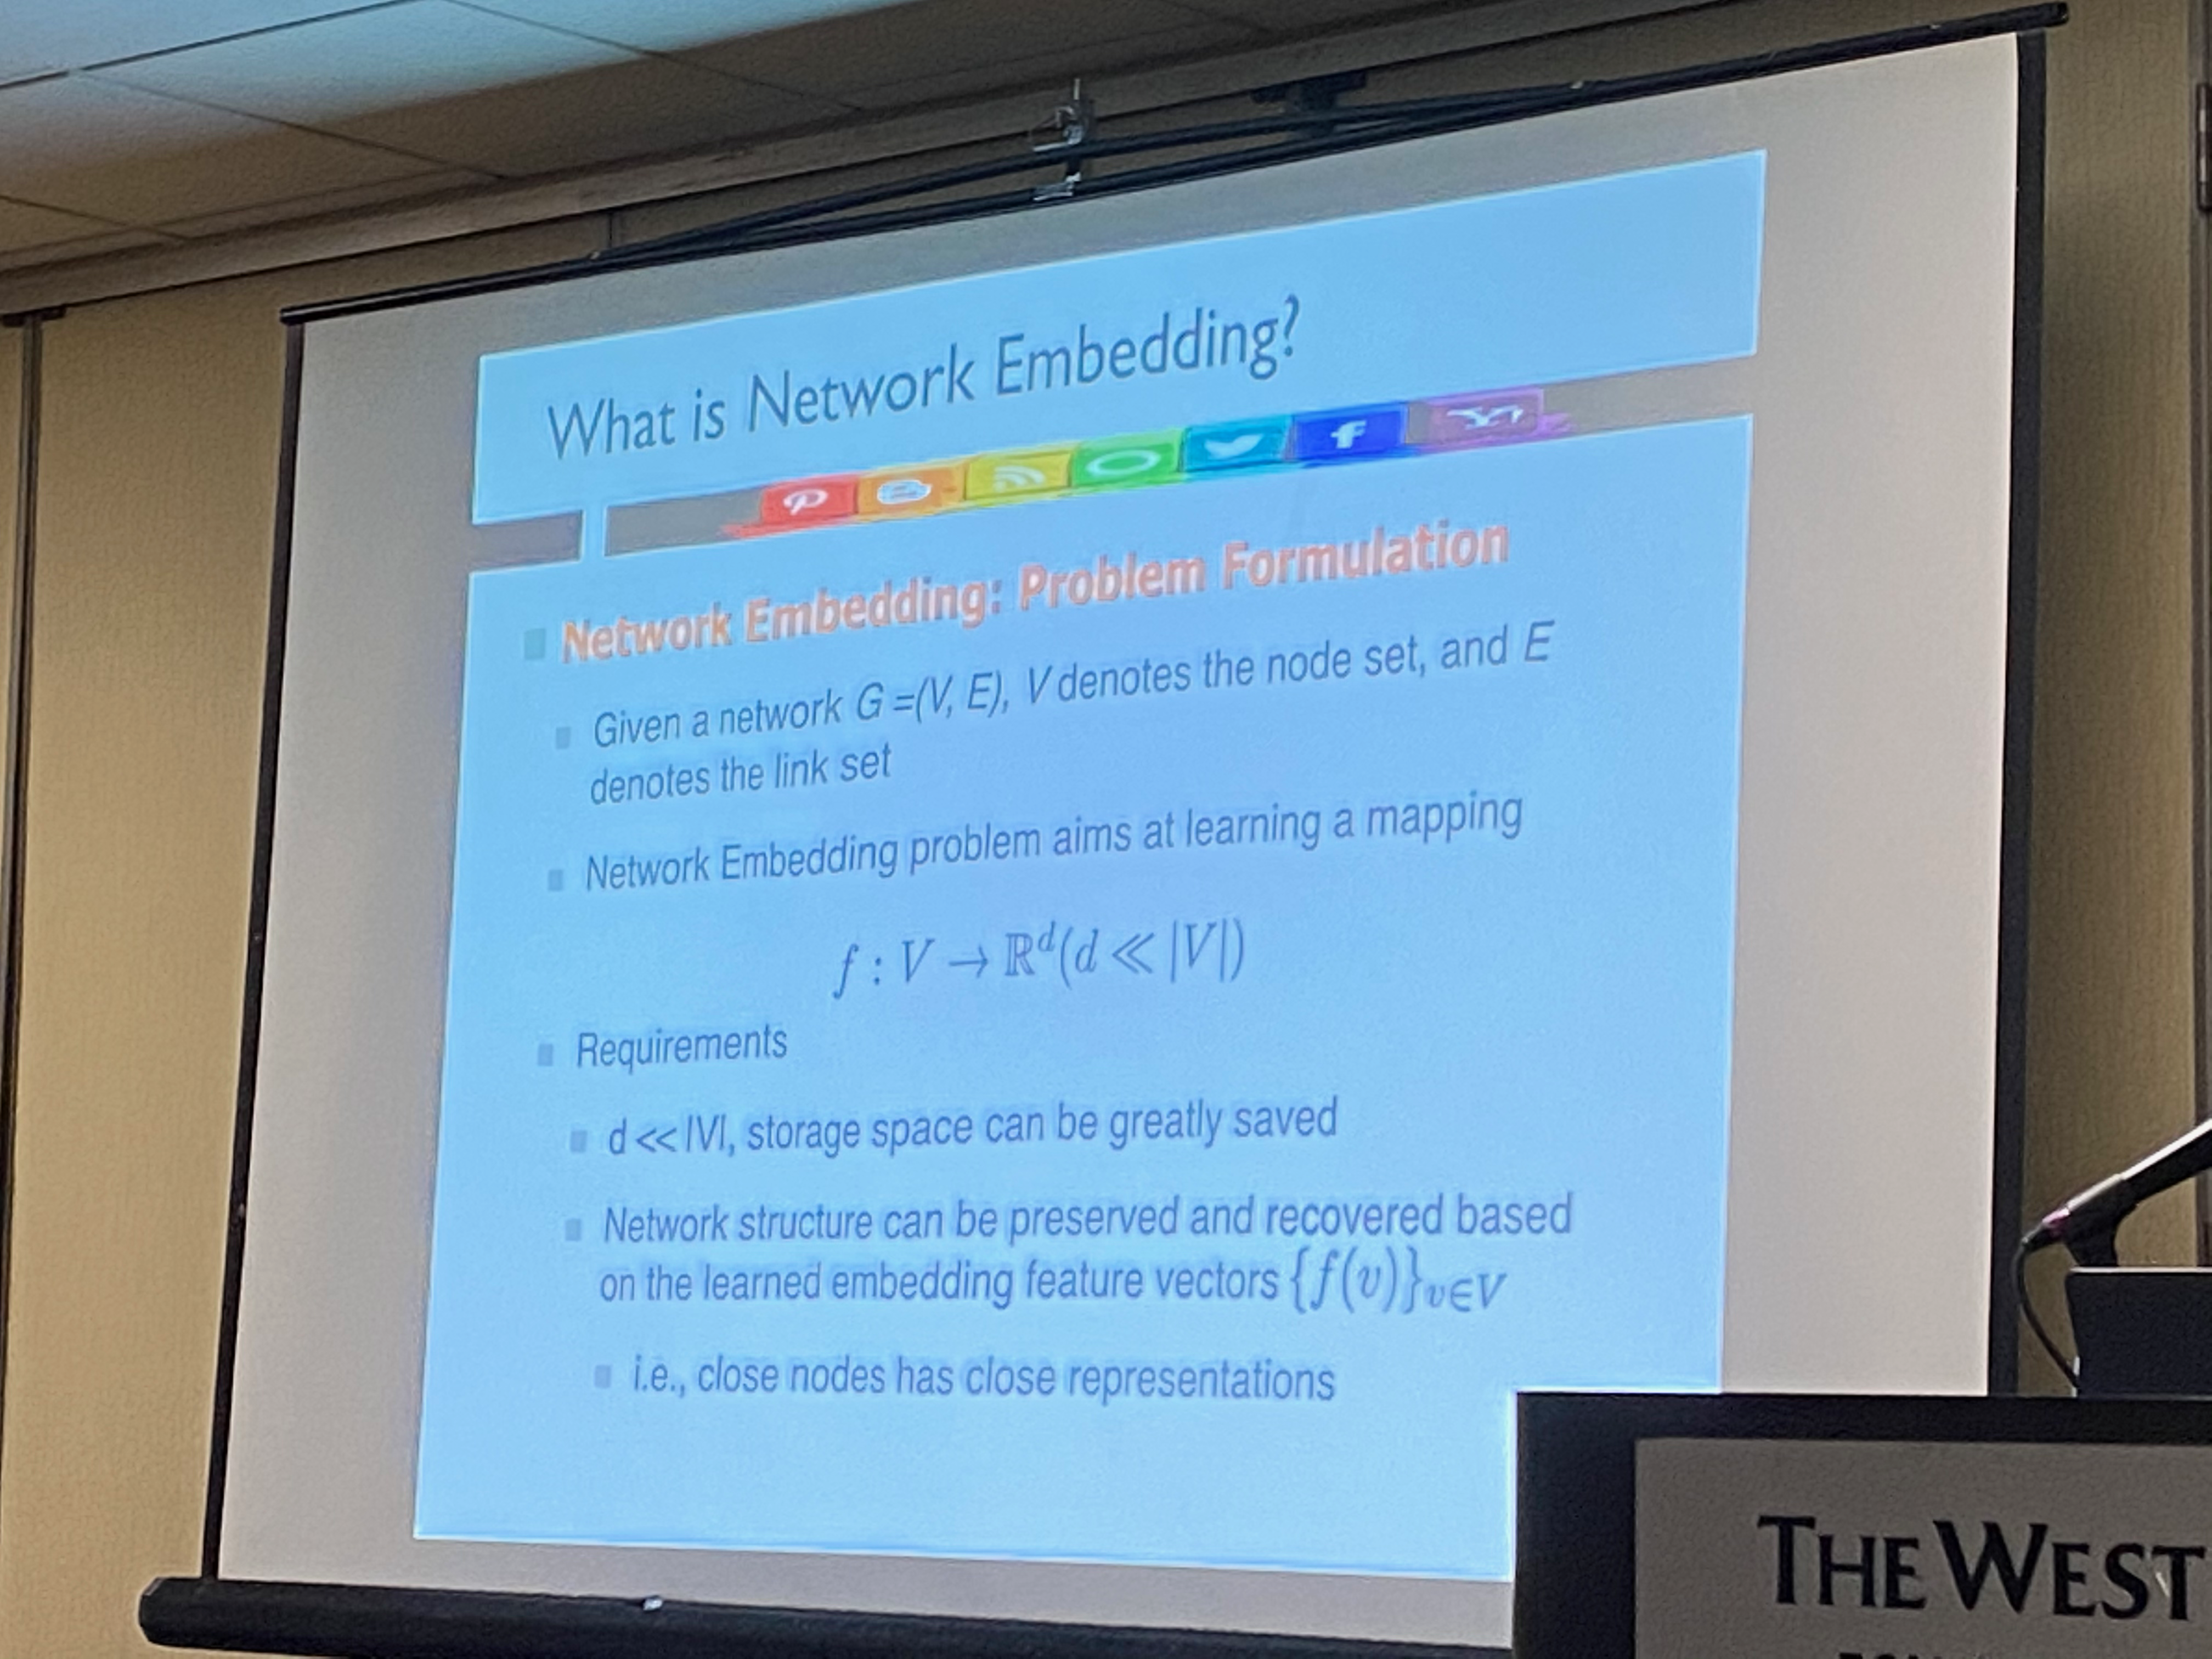
\includegraphics[width=120mm]{images/network_embedding.png}
    \caption{Network embedding}
    \label{fig:my_label}
\end{figure}{}


\subsubsection{BIGMat: A distributed affinity-perserving random walk strategy for instance mathcing on knowledge graph}

$\ra$ essentially a link prediction in knowledge graph by doing instance matching. Two nodes are matching candidate if they share at least one word, but this seems to be a big drawback.

\subsubsection{RecANt: Network-based Recruitment for Active Fake news Correction}

\begin{figure}[ht!]
    \centering
    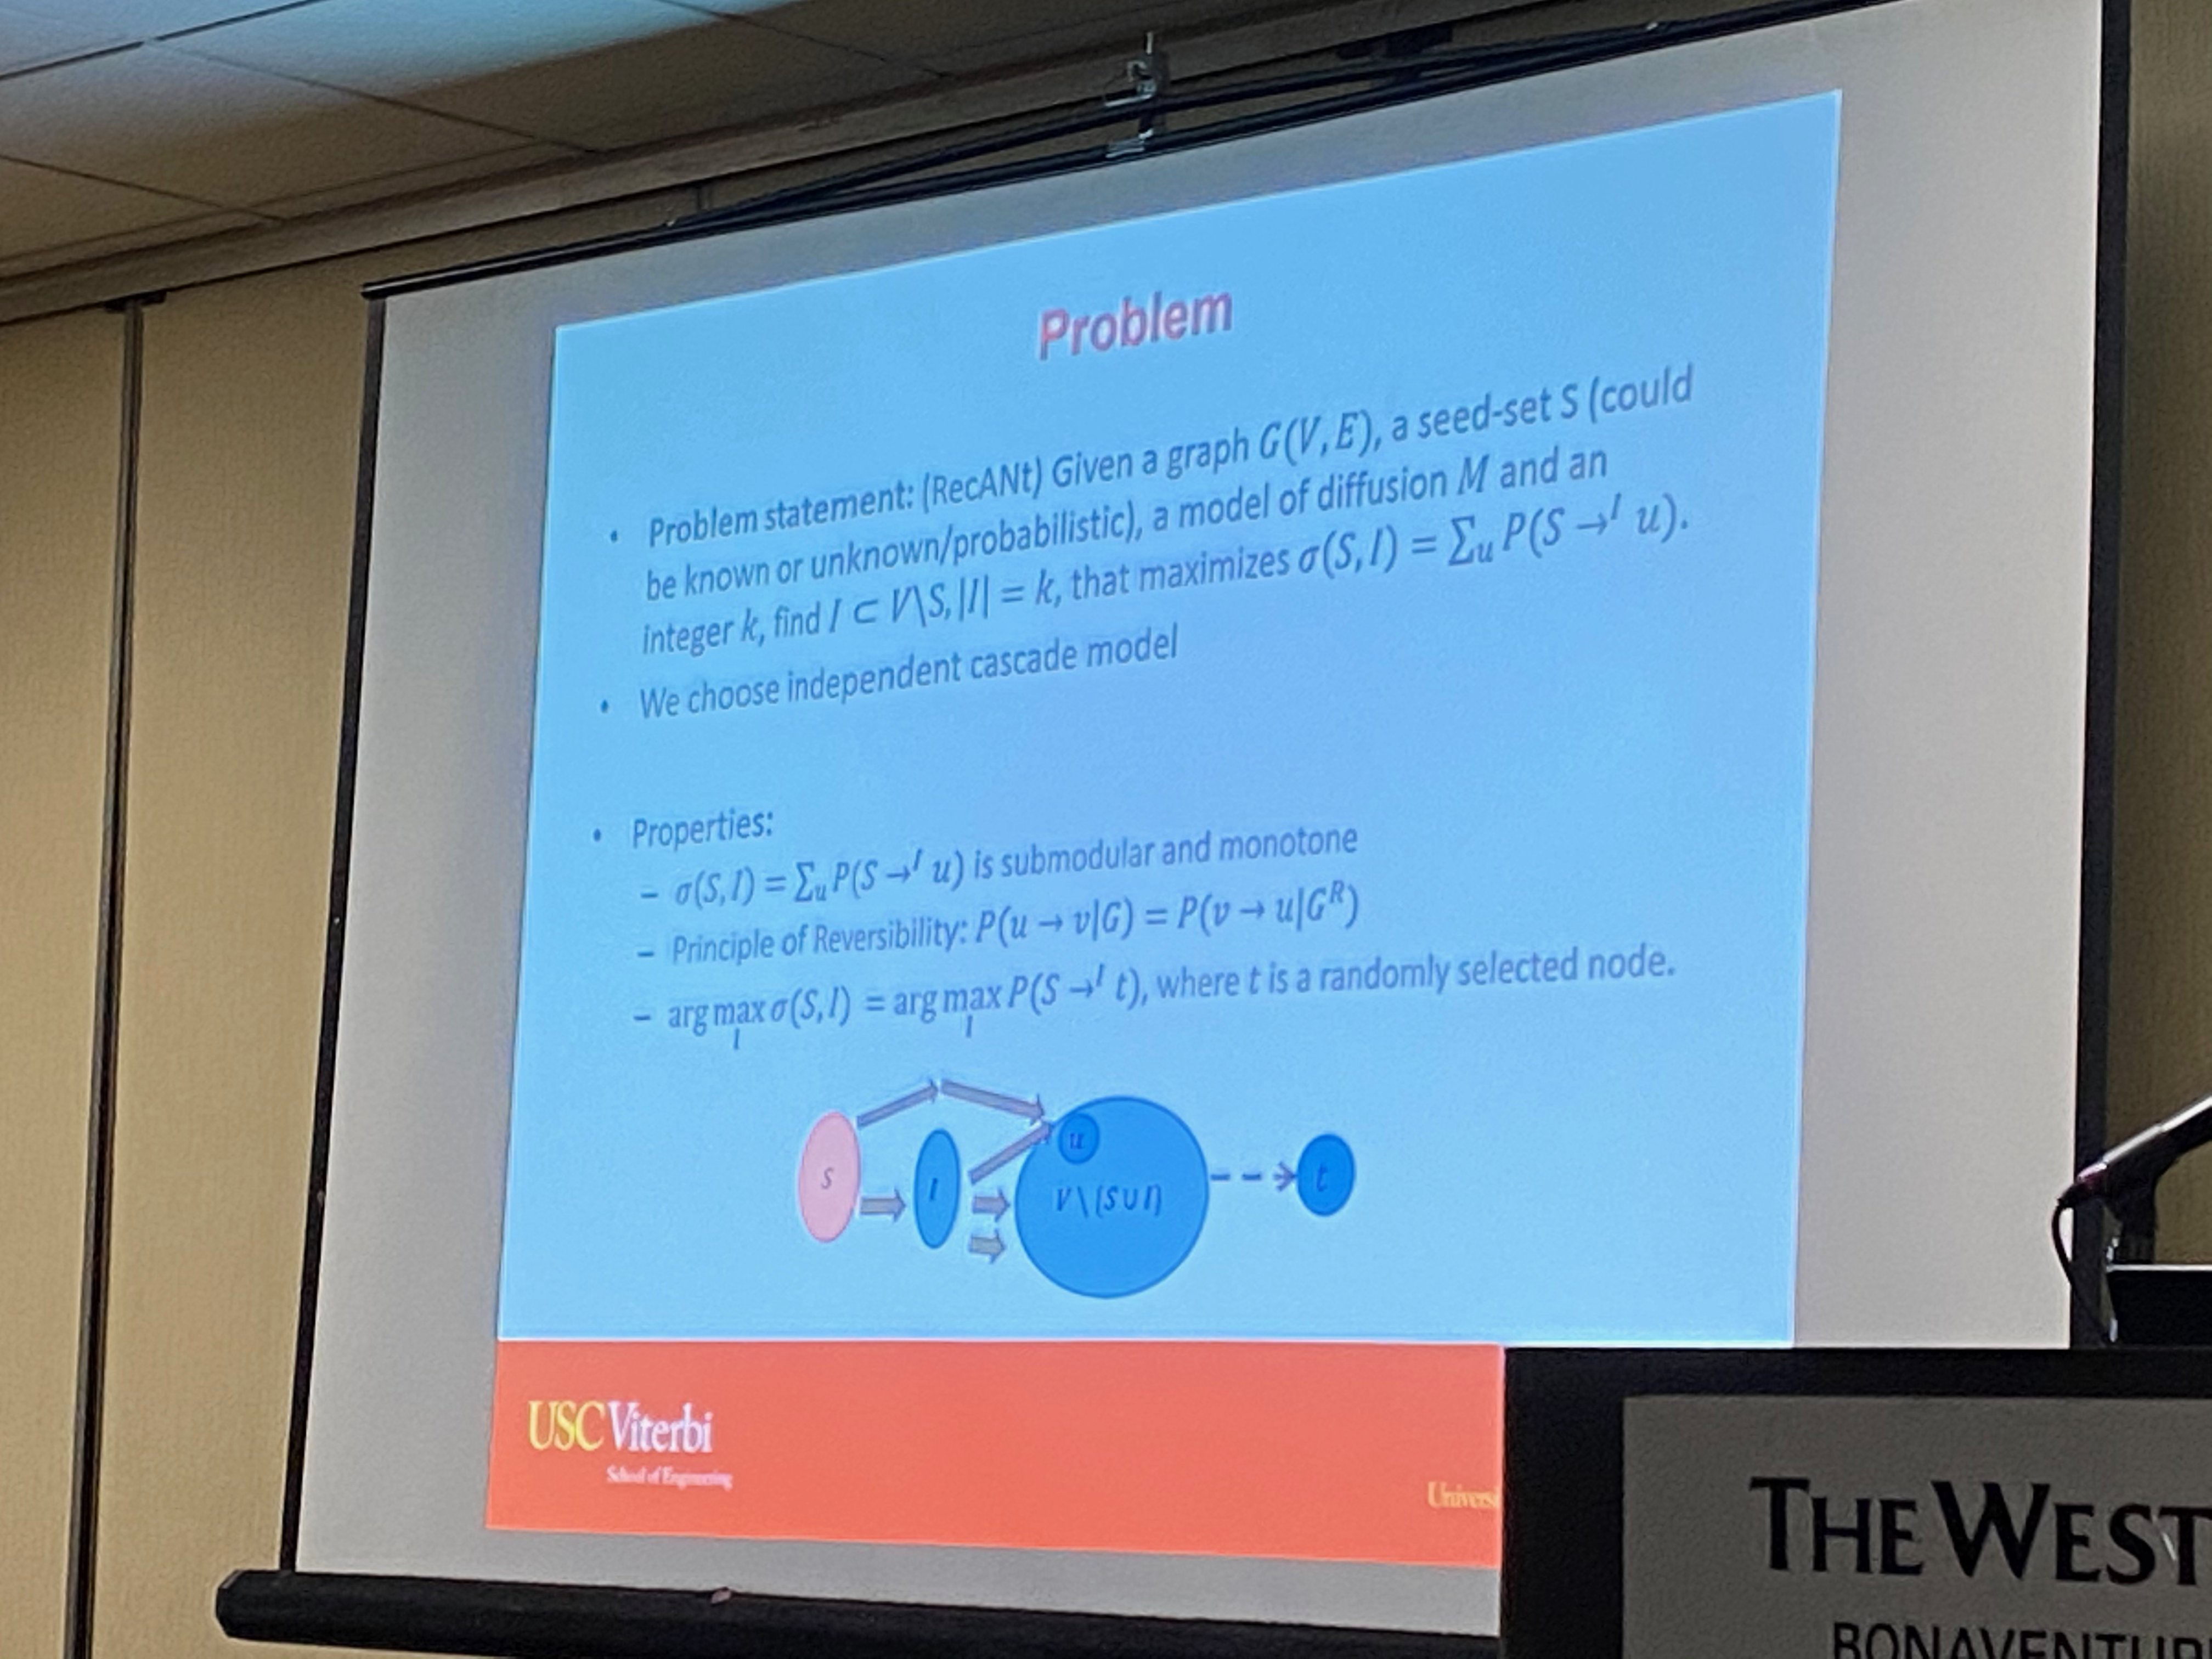
\includegraphics[width=120mm]{images/fake_news_prob.png}
    \caption{Network embedding}
    \label{fig:my_label}
\end{figure}{}

\begin{figure}[ht!]
    \centering
    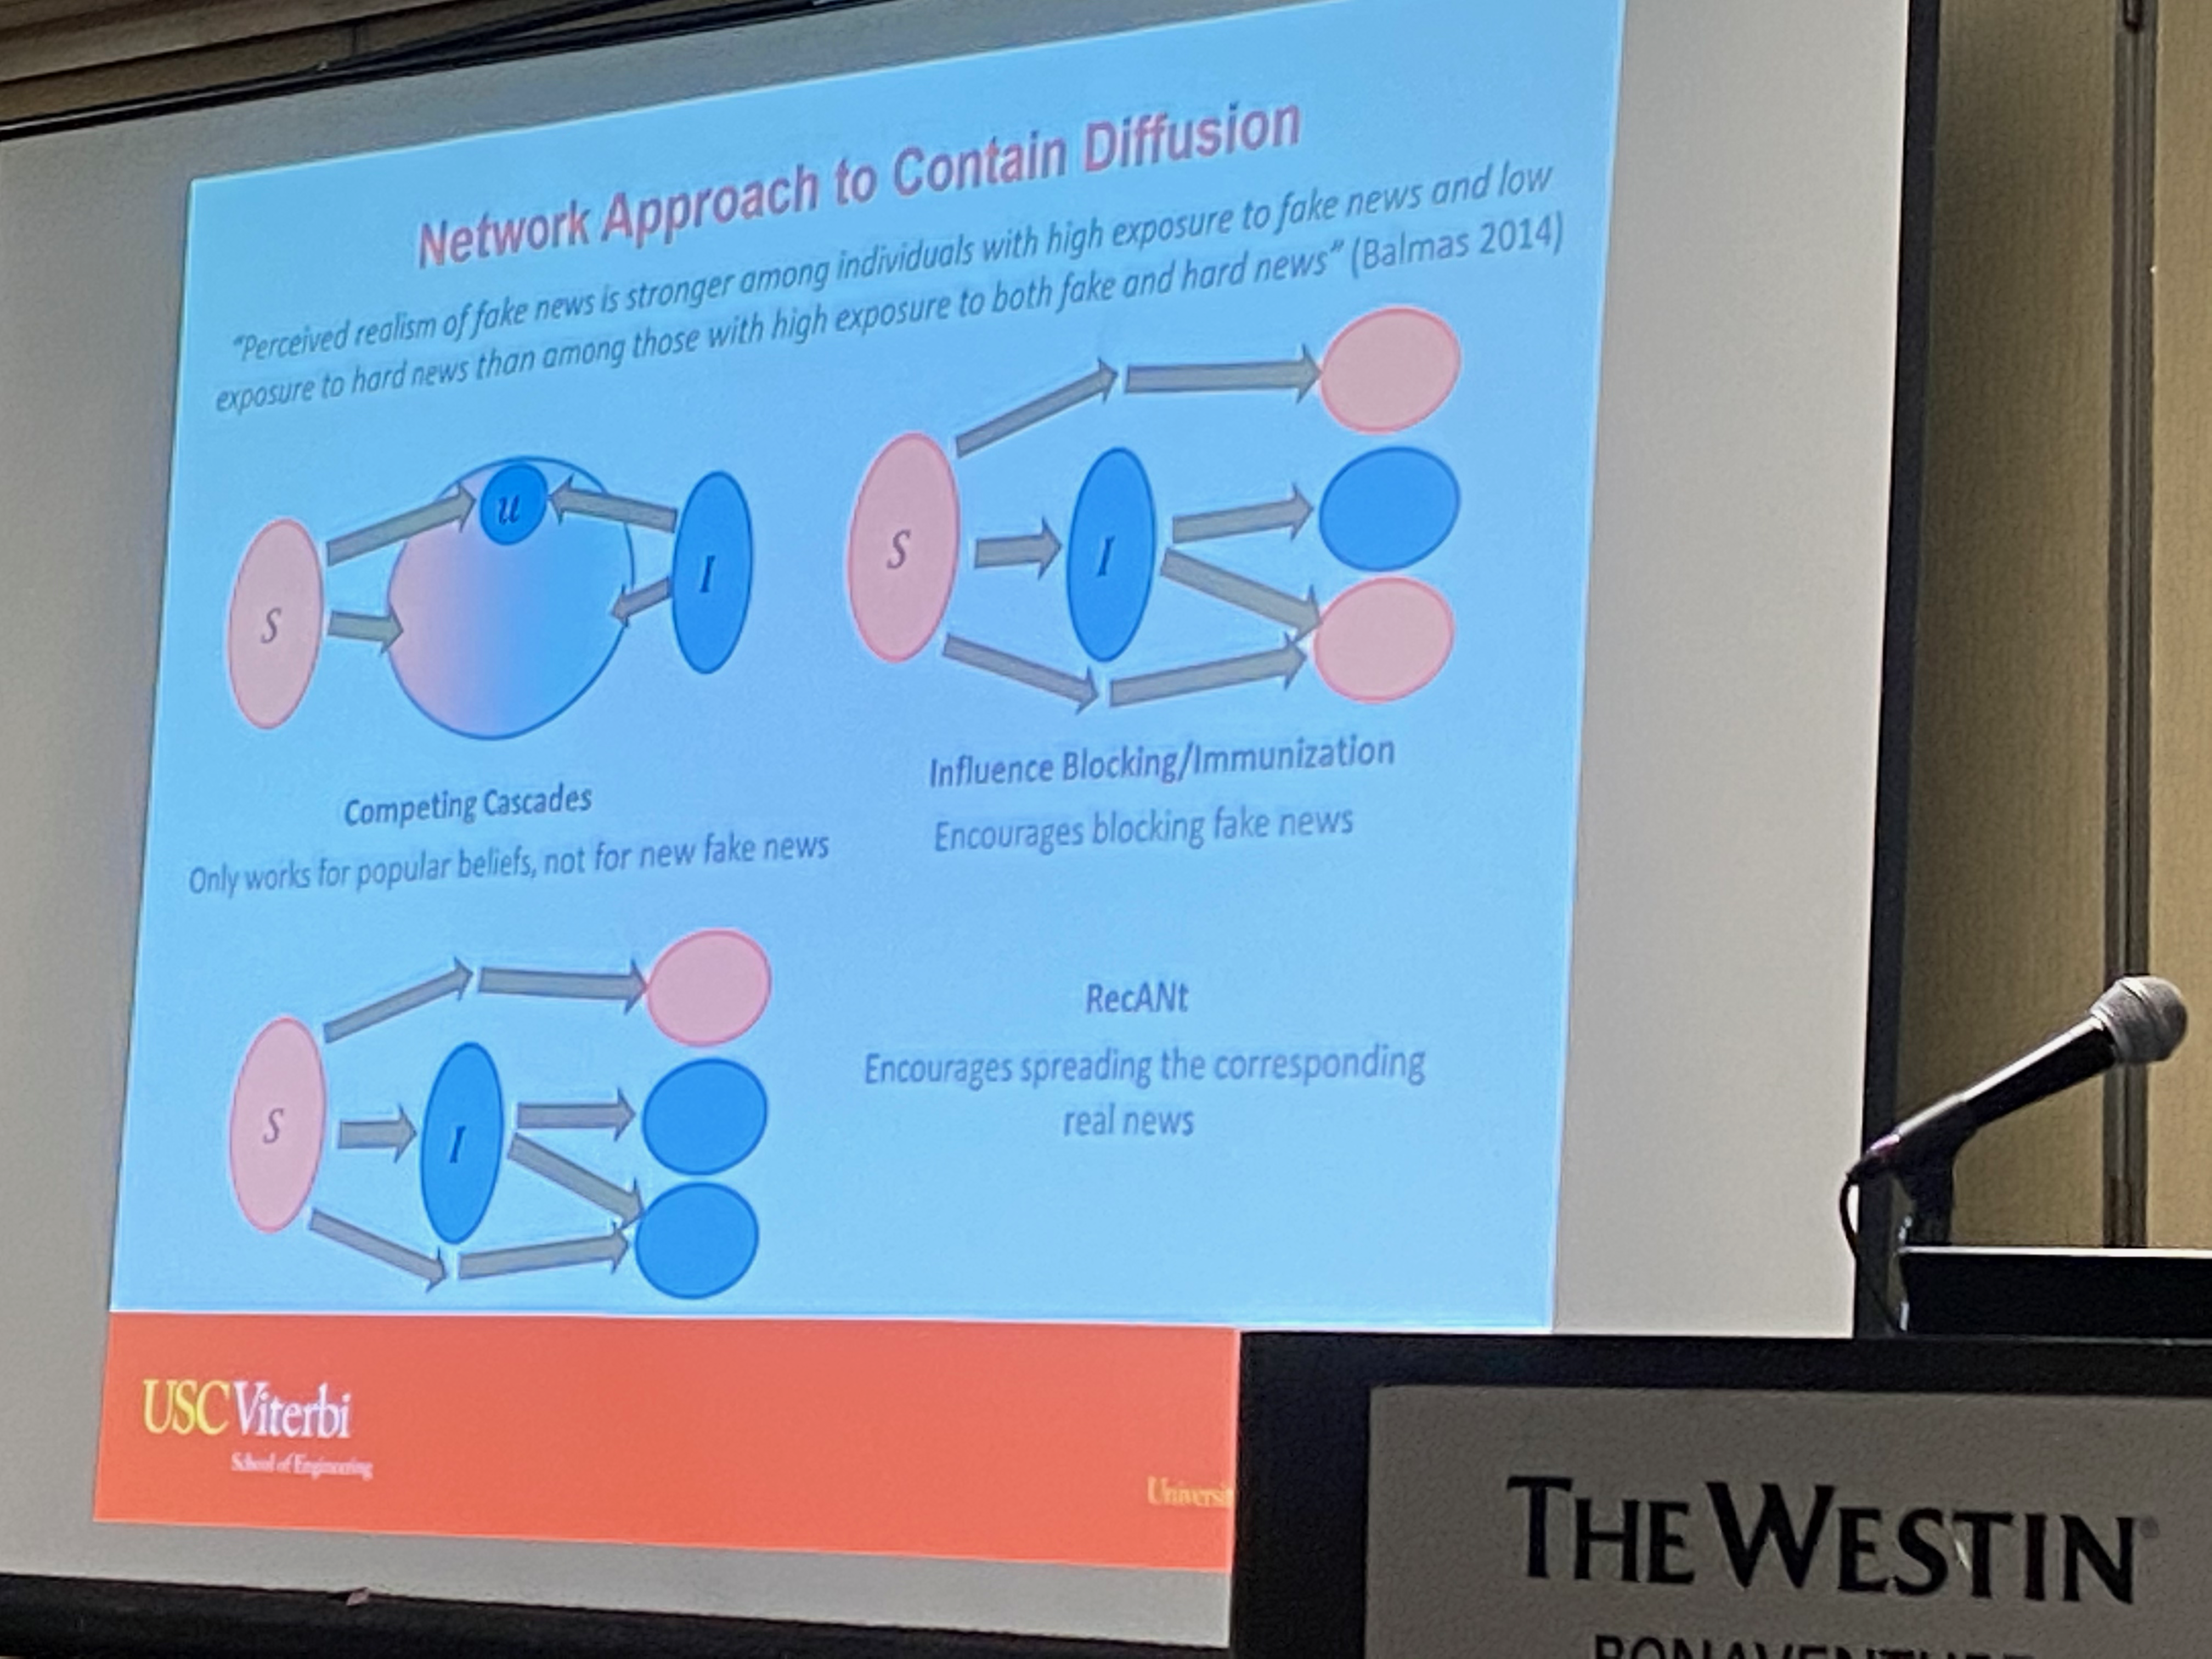
\includegraphics[width=120mm]{images/fake_news_diffusion.png}
    \caption{Network embedding}
    \label{fig:my_label}
\end{figure}{}

\subsubsection{Modelling Online Comment Threads from their Start}

{\bf Comment threads: take the form of a tree. The root is the original post. Comments are descendants of root}

\remark{Why we are trying to predict the comment threads?}

\begin{figure}
    \centering
    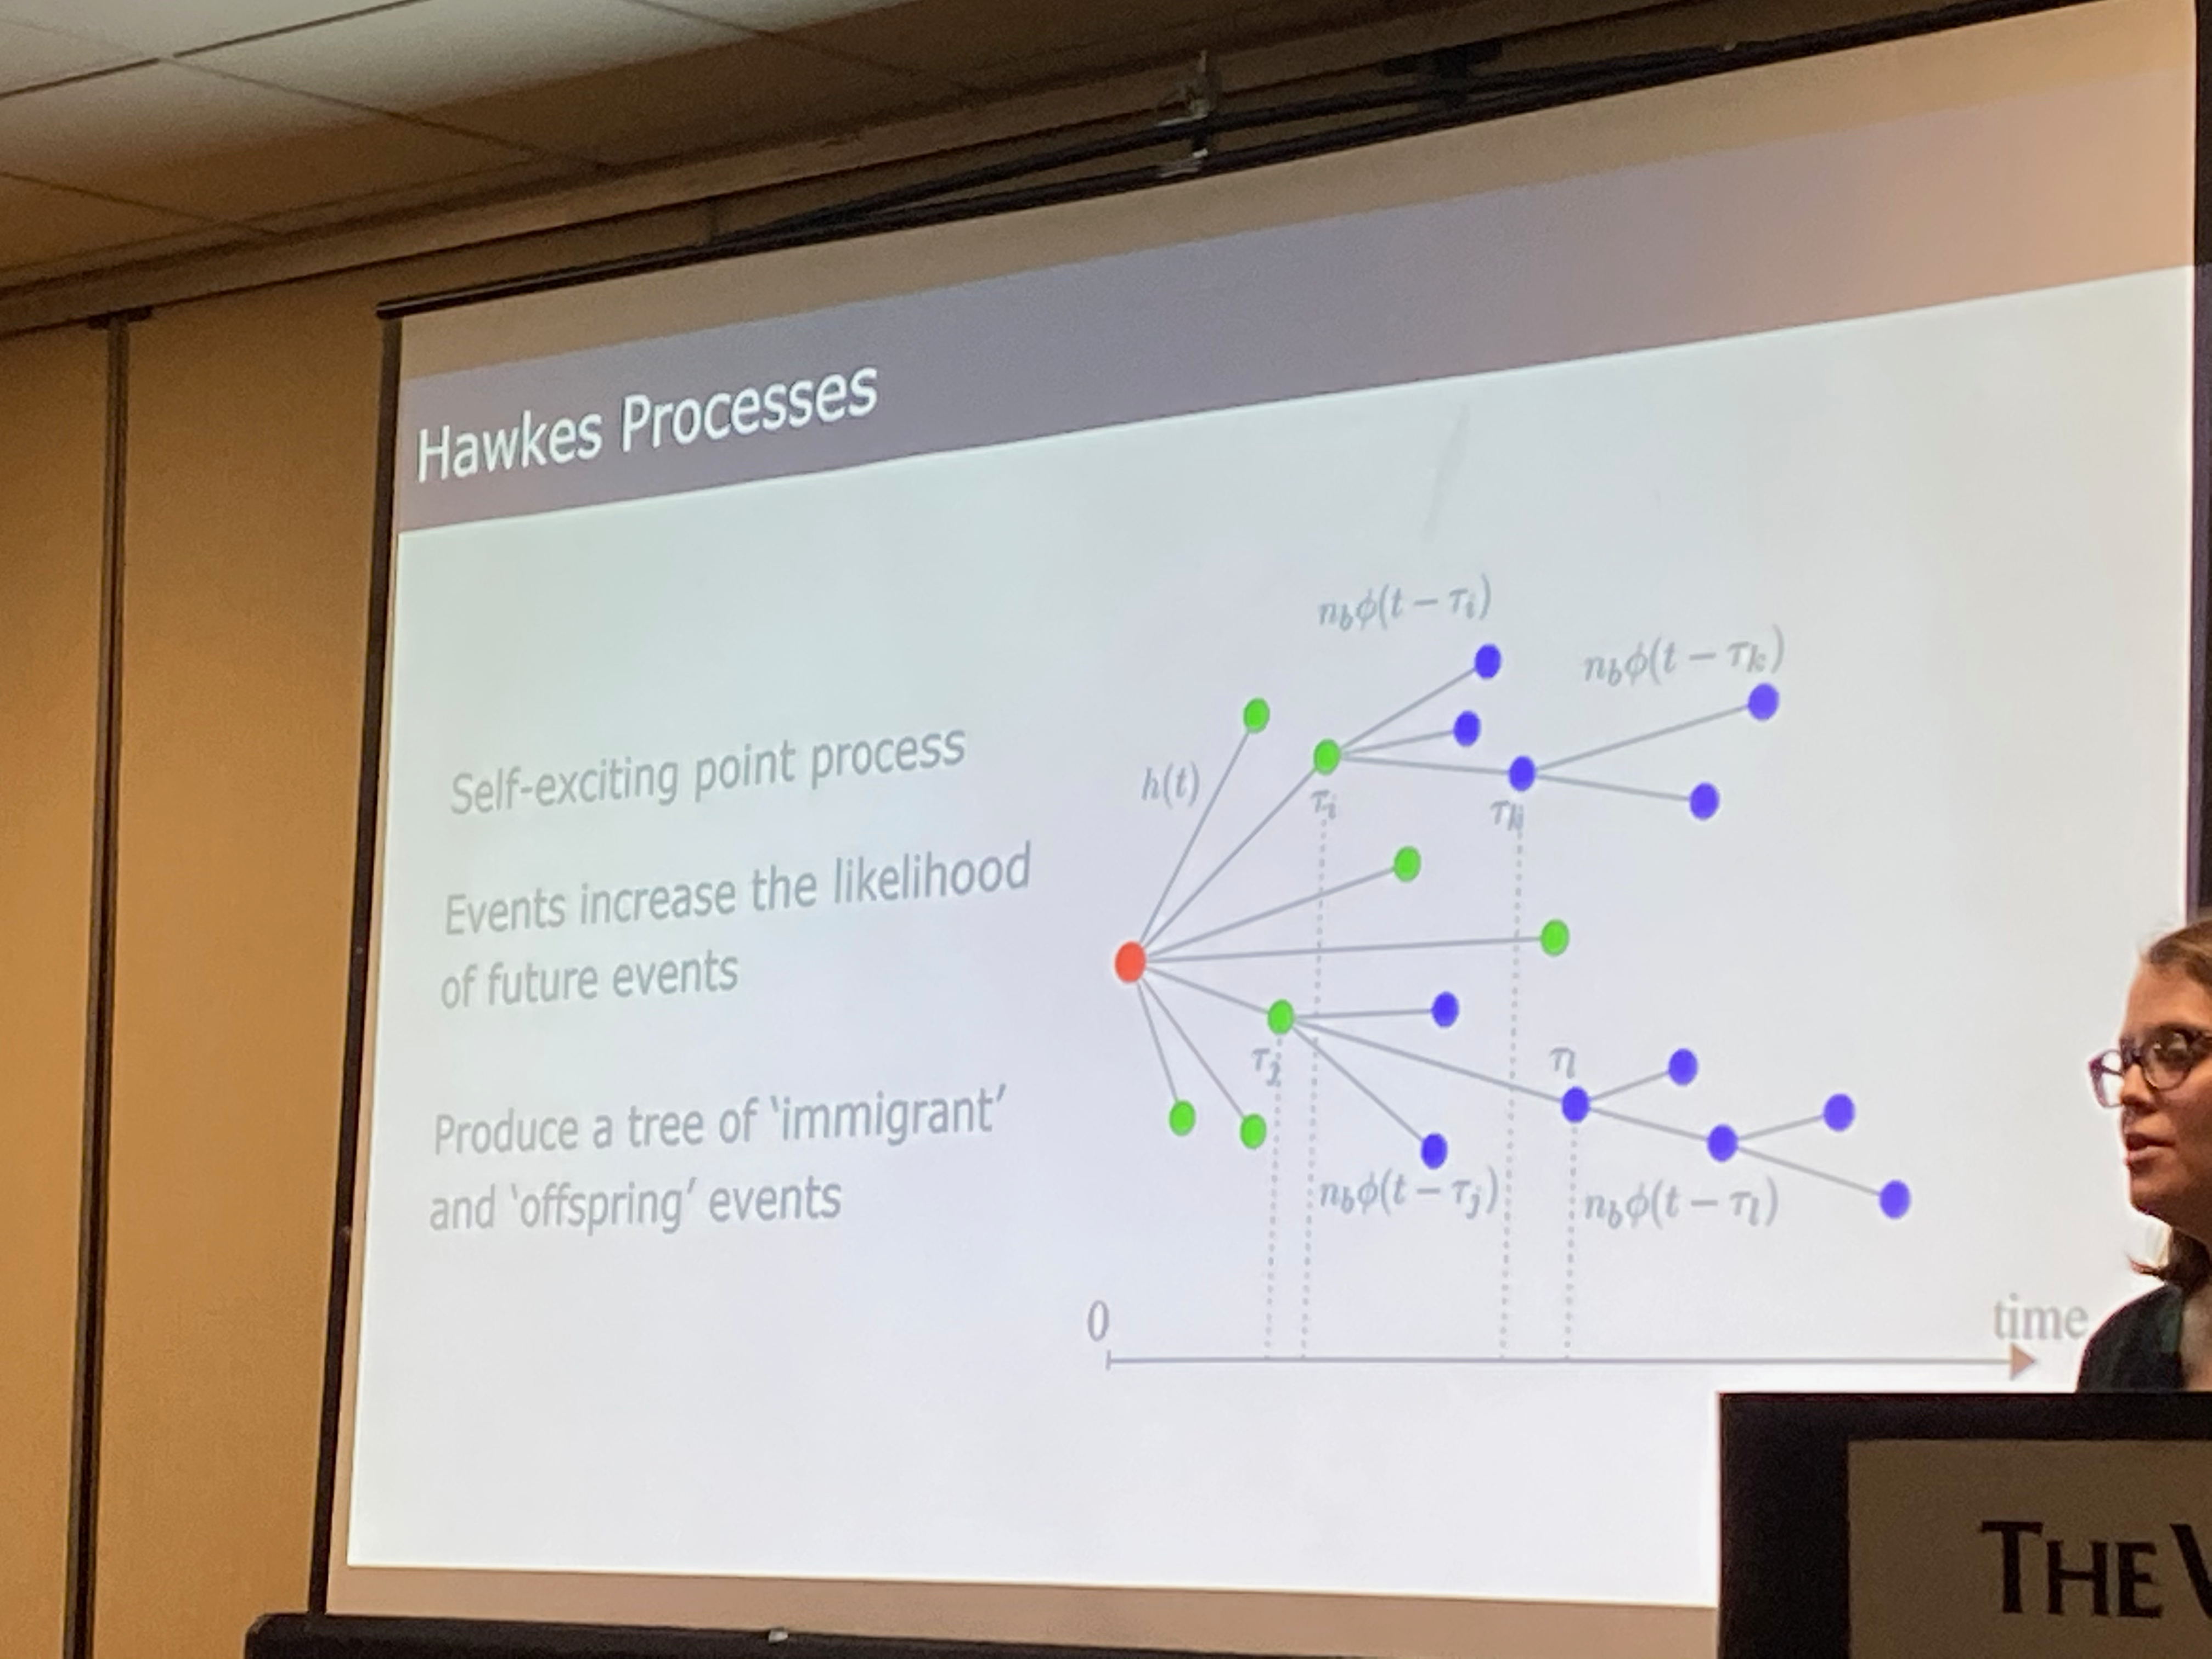
\includegraphics[width=120mm]{images/hawks.png}
    \caption{Hawks process}
    \label{fig:my_label}
\end{figure}{}

\begin{figure}
    \centering
    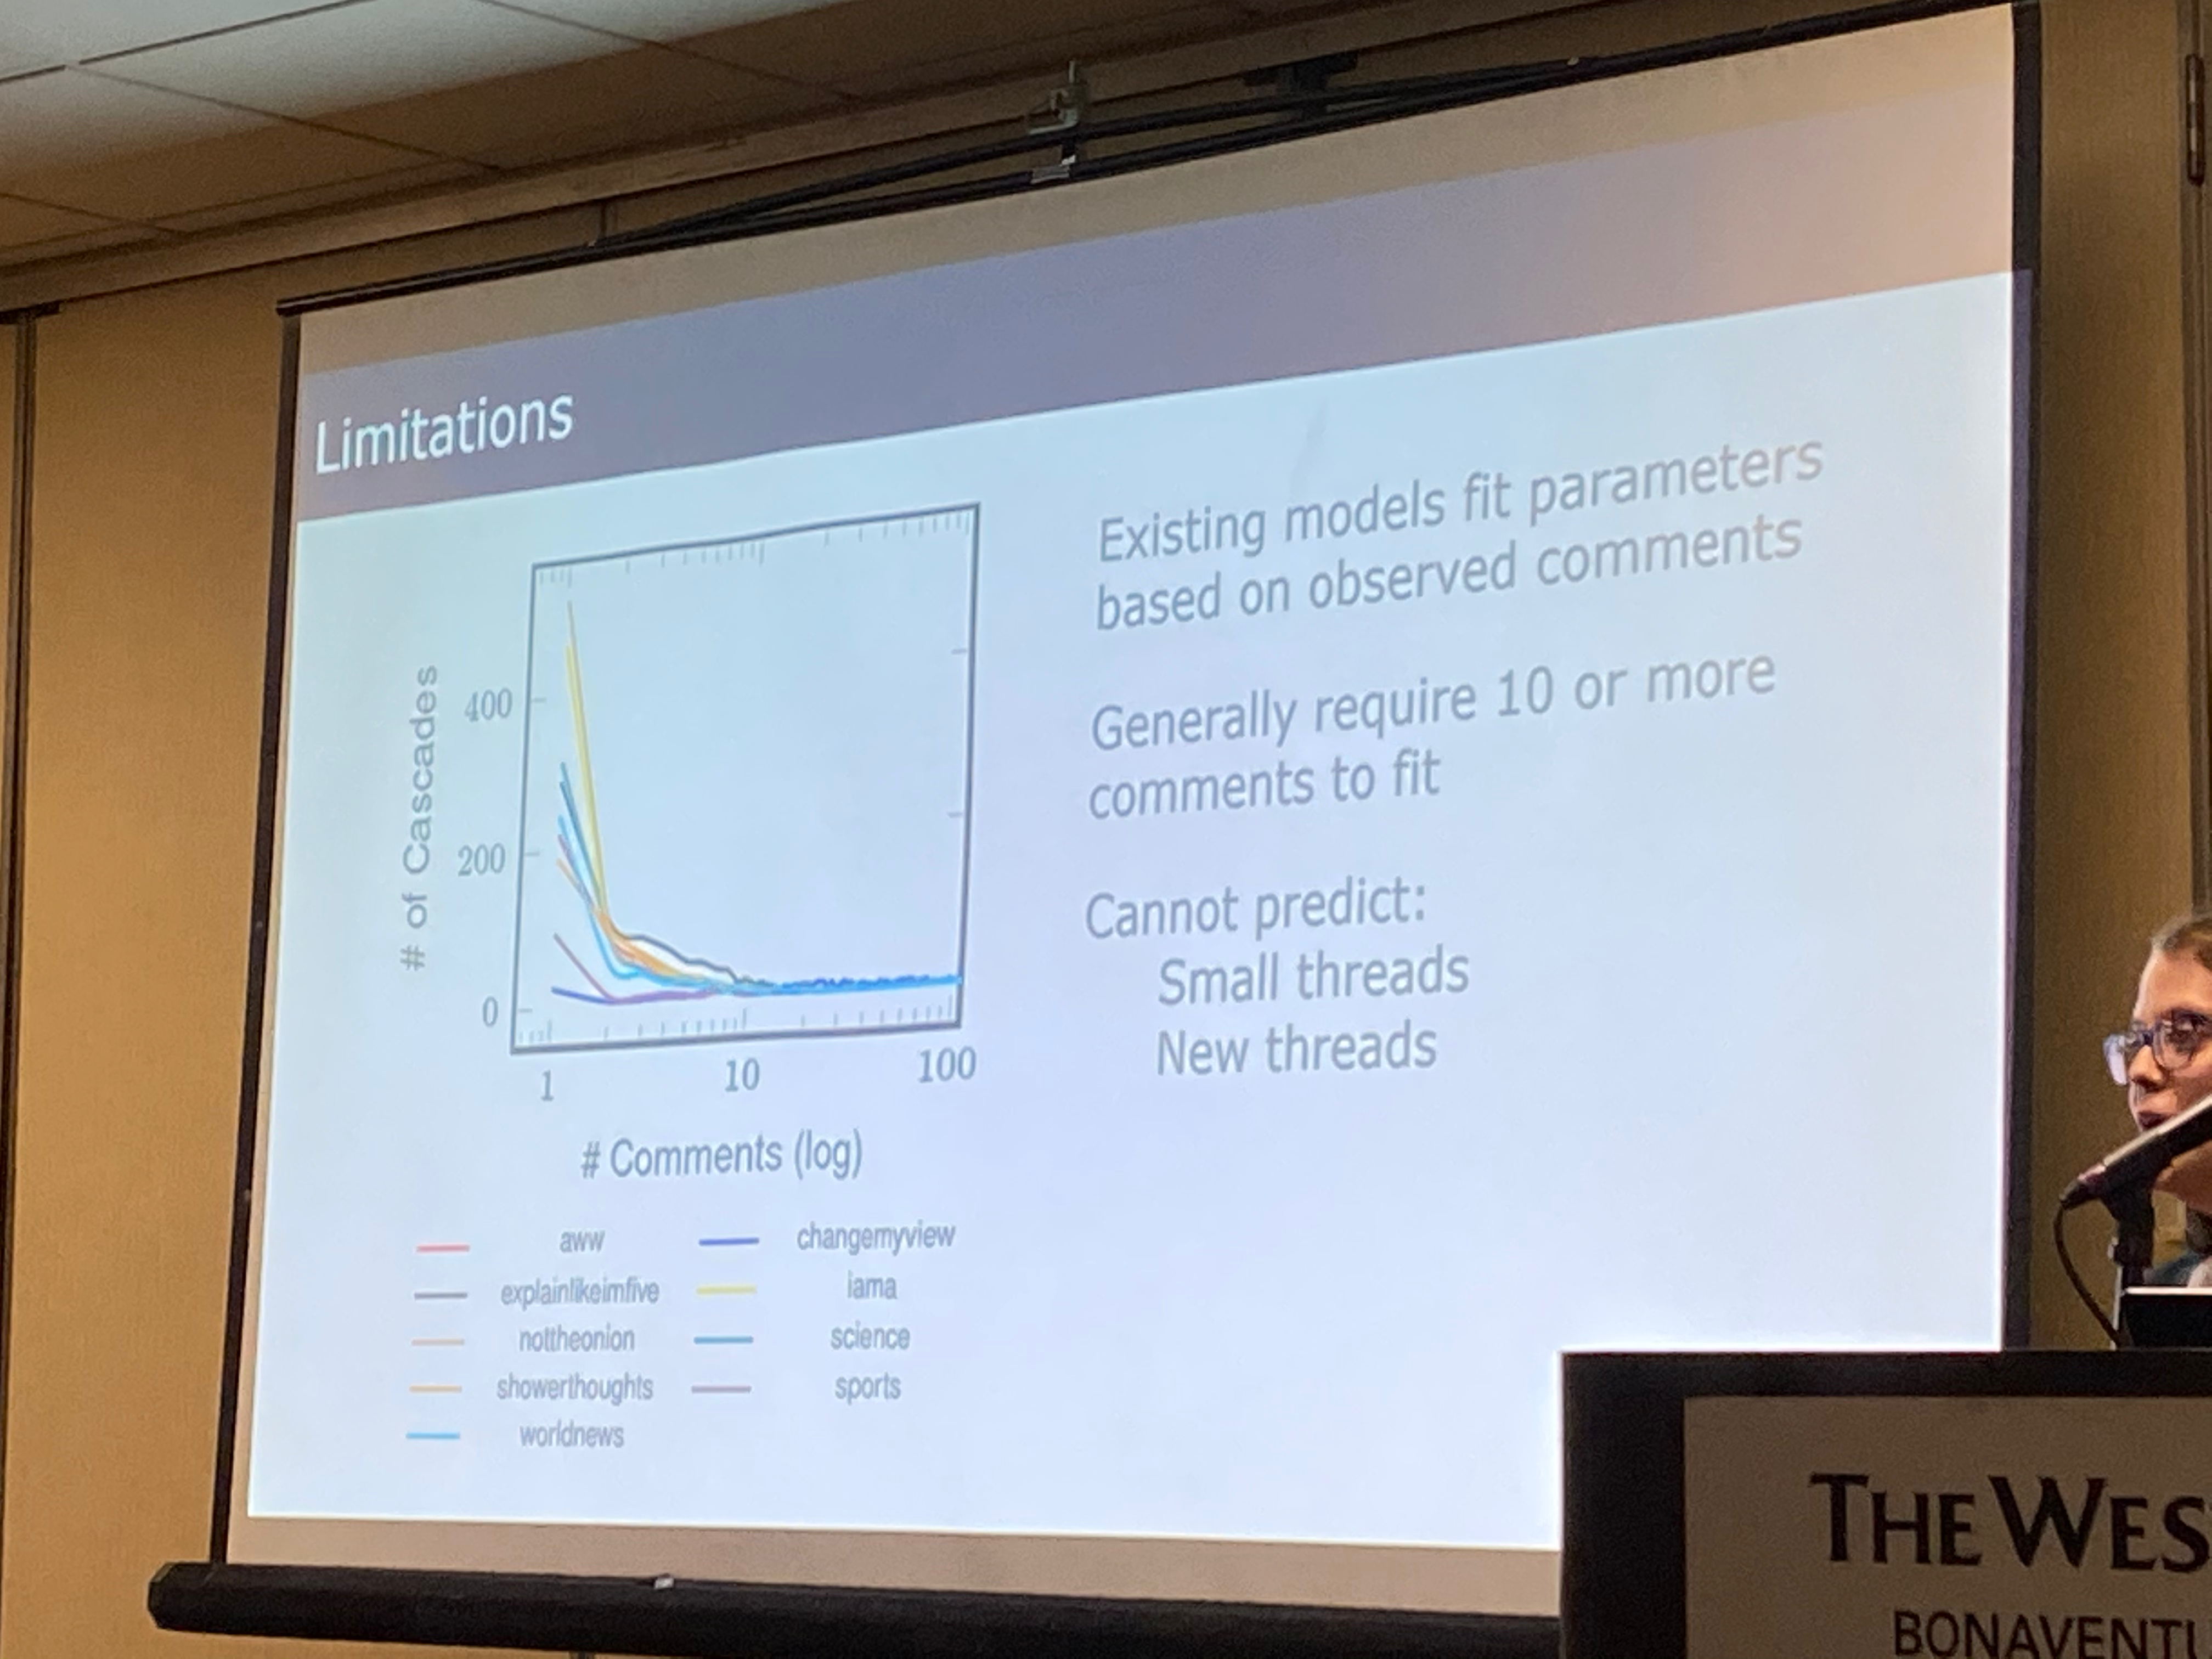
\includegraphics[width=120mm]{images/hawks_lim.png}
    \caption{Limitations of hawks process}
    \label{fig:my_label}
\end{figure}{}

\subsubsection{Improving Scalability of Parallel CNN Training by Adjusting Mini-Batch Size at Run-Time}

{\bf Challenge:} Training modern CNN models requires too much computing time which sometime hinders the practicality of new CNN models. Thus, parallel training is often adopted.

\begin{figure}
    \centering
    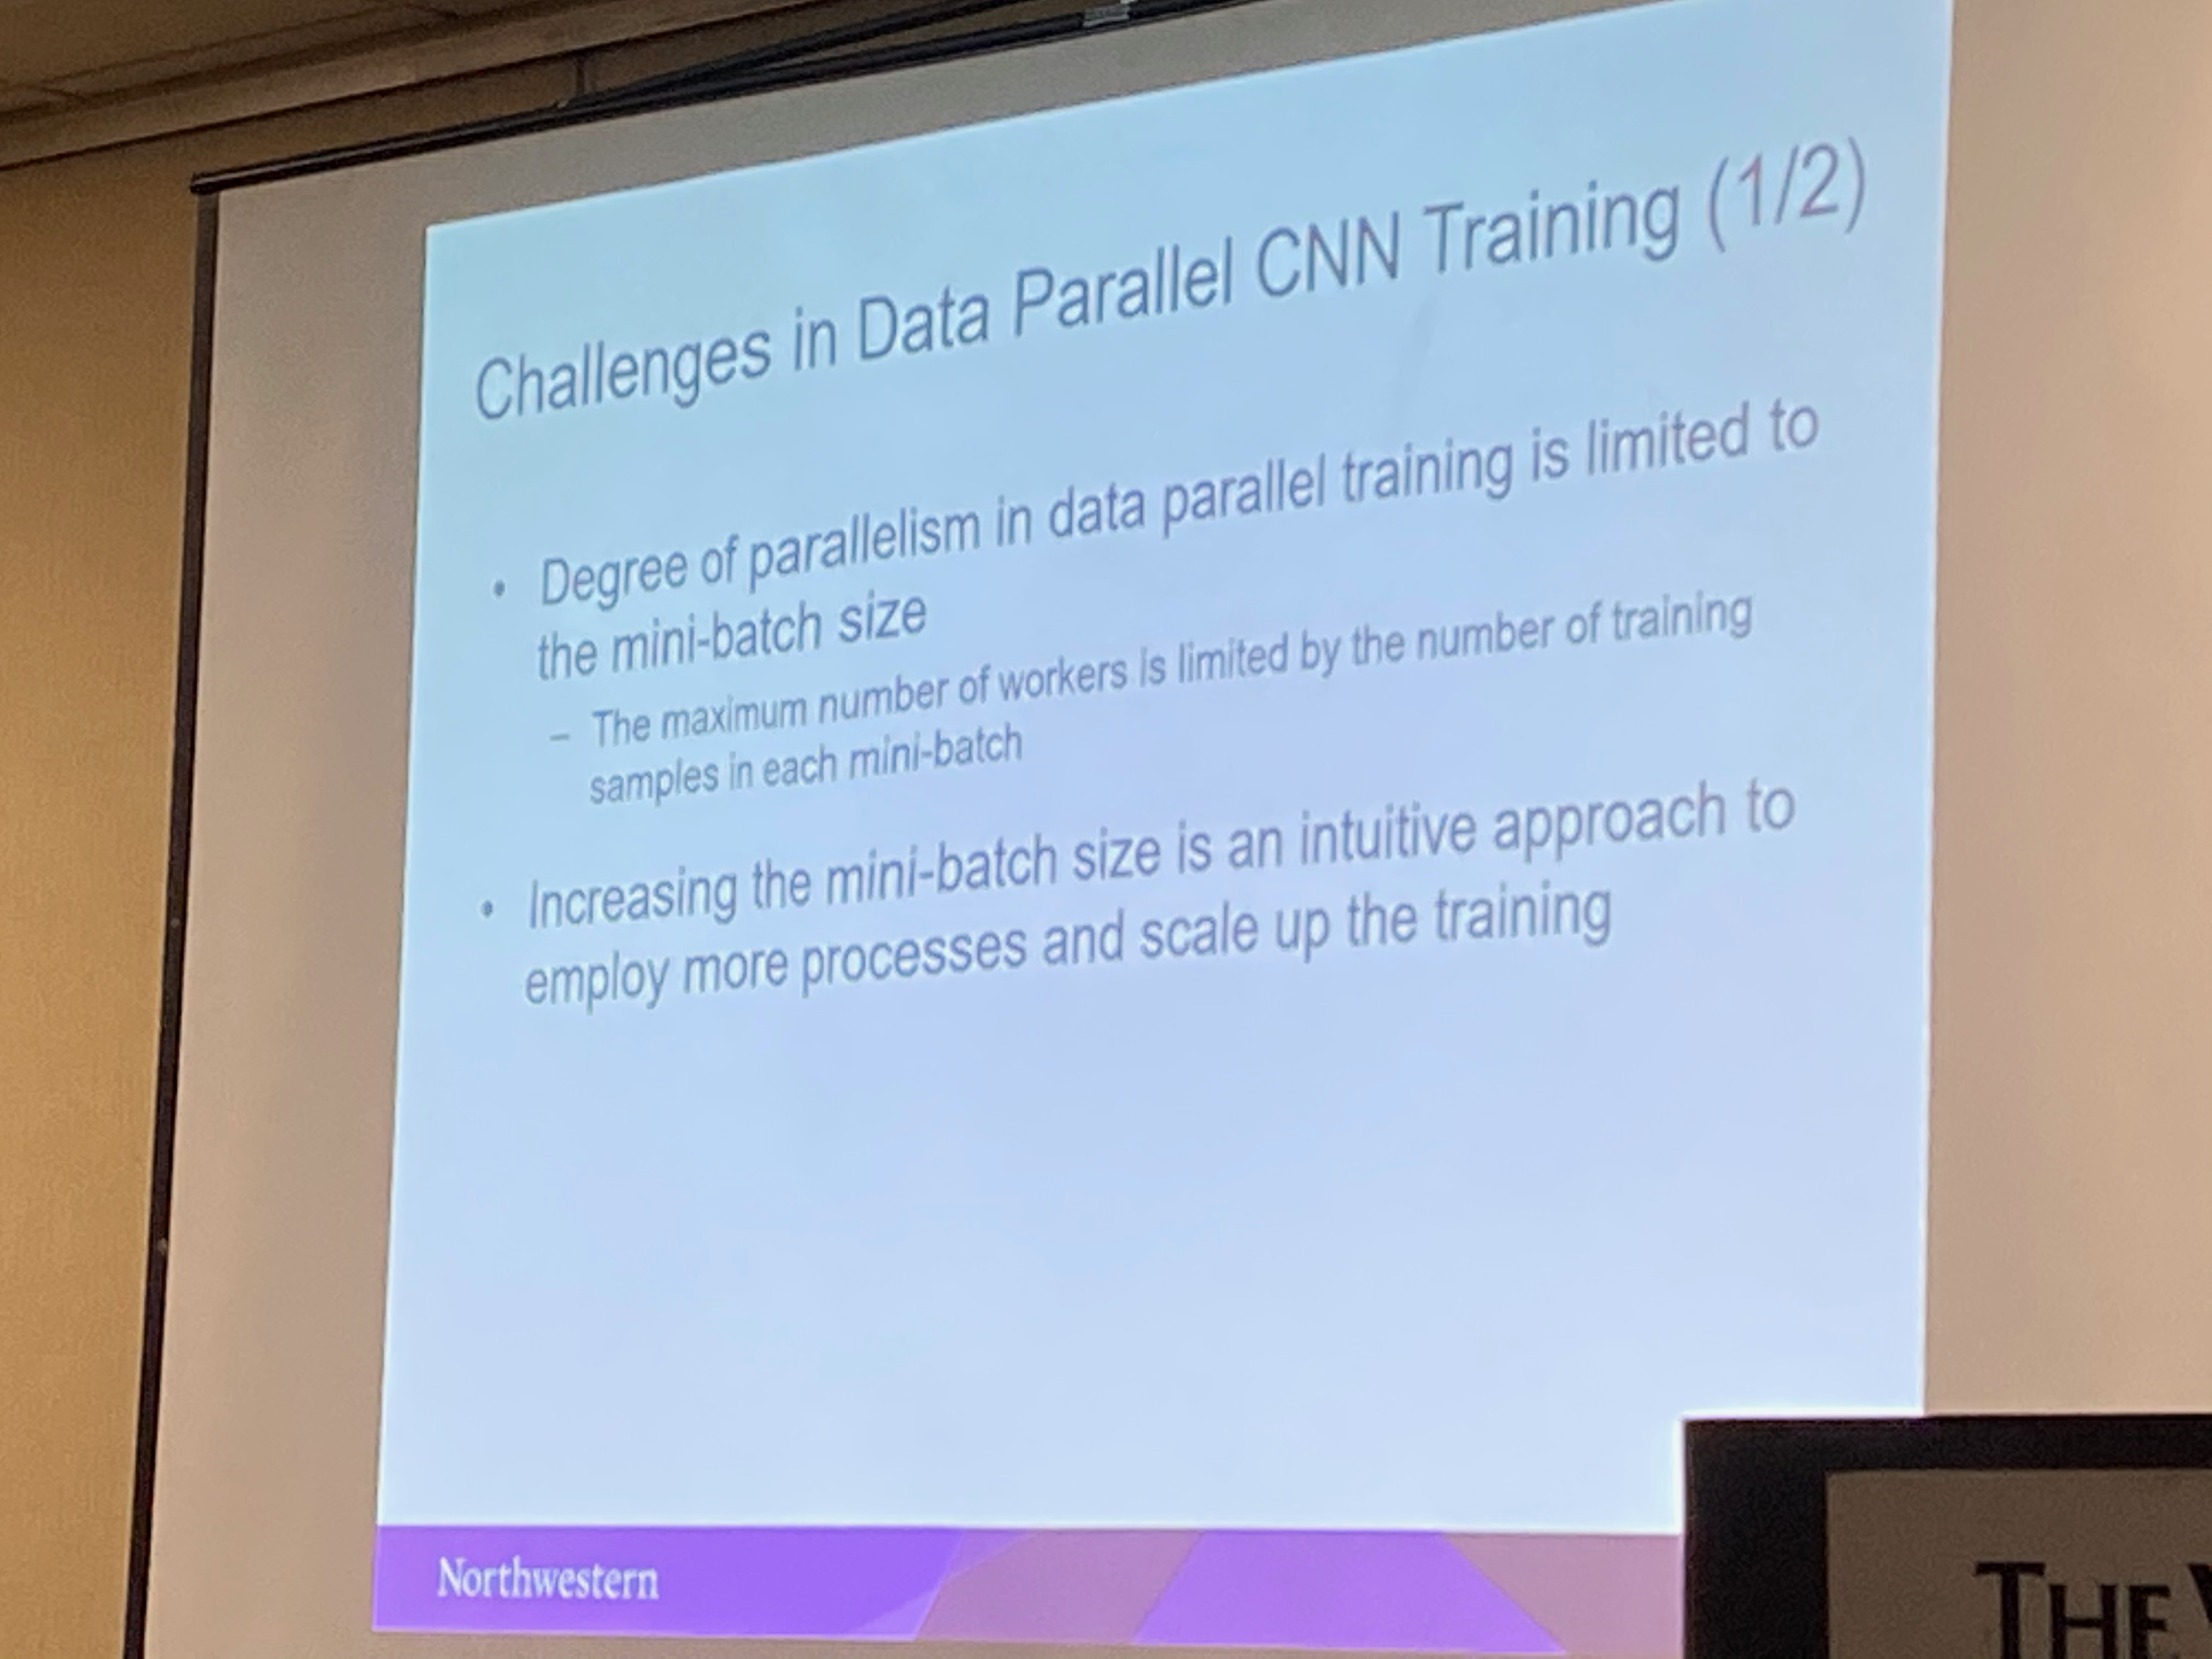
\includegraphics[width=120mm]{images/cnn_parallel.png}
    \caption{Data parallel CNN training}
    \label{fig:my_label}
\end{figure}{}

\begin{figure}
    \centering
    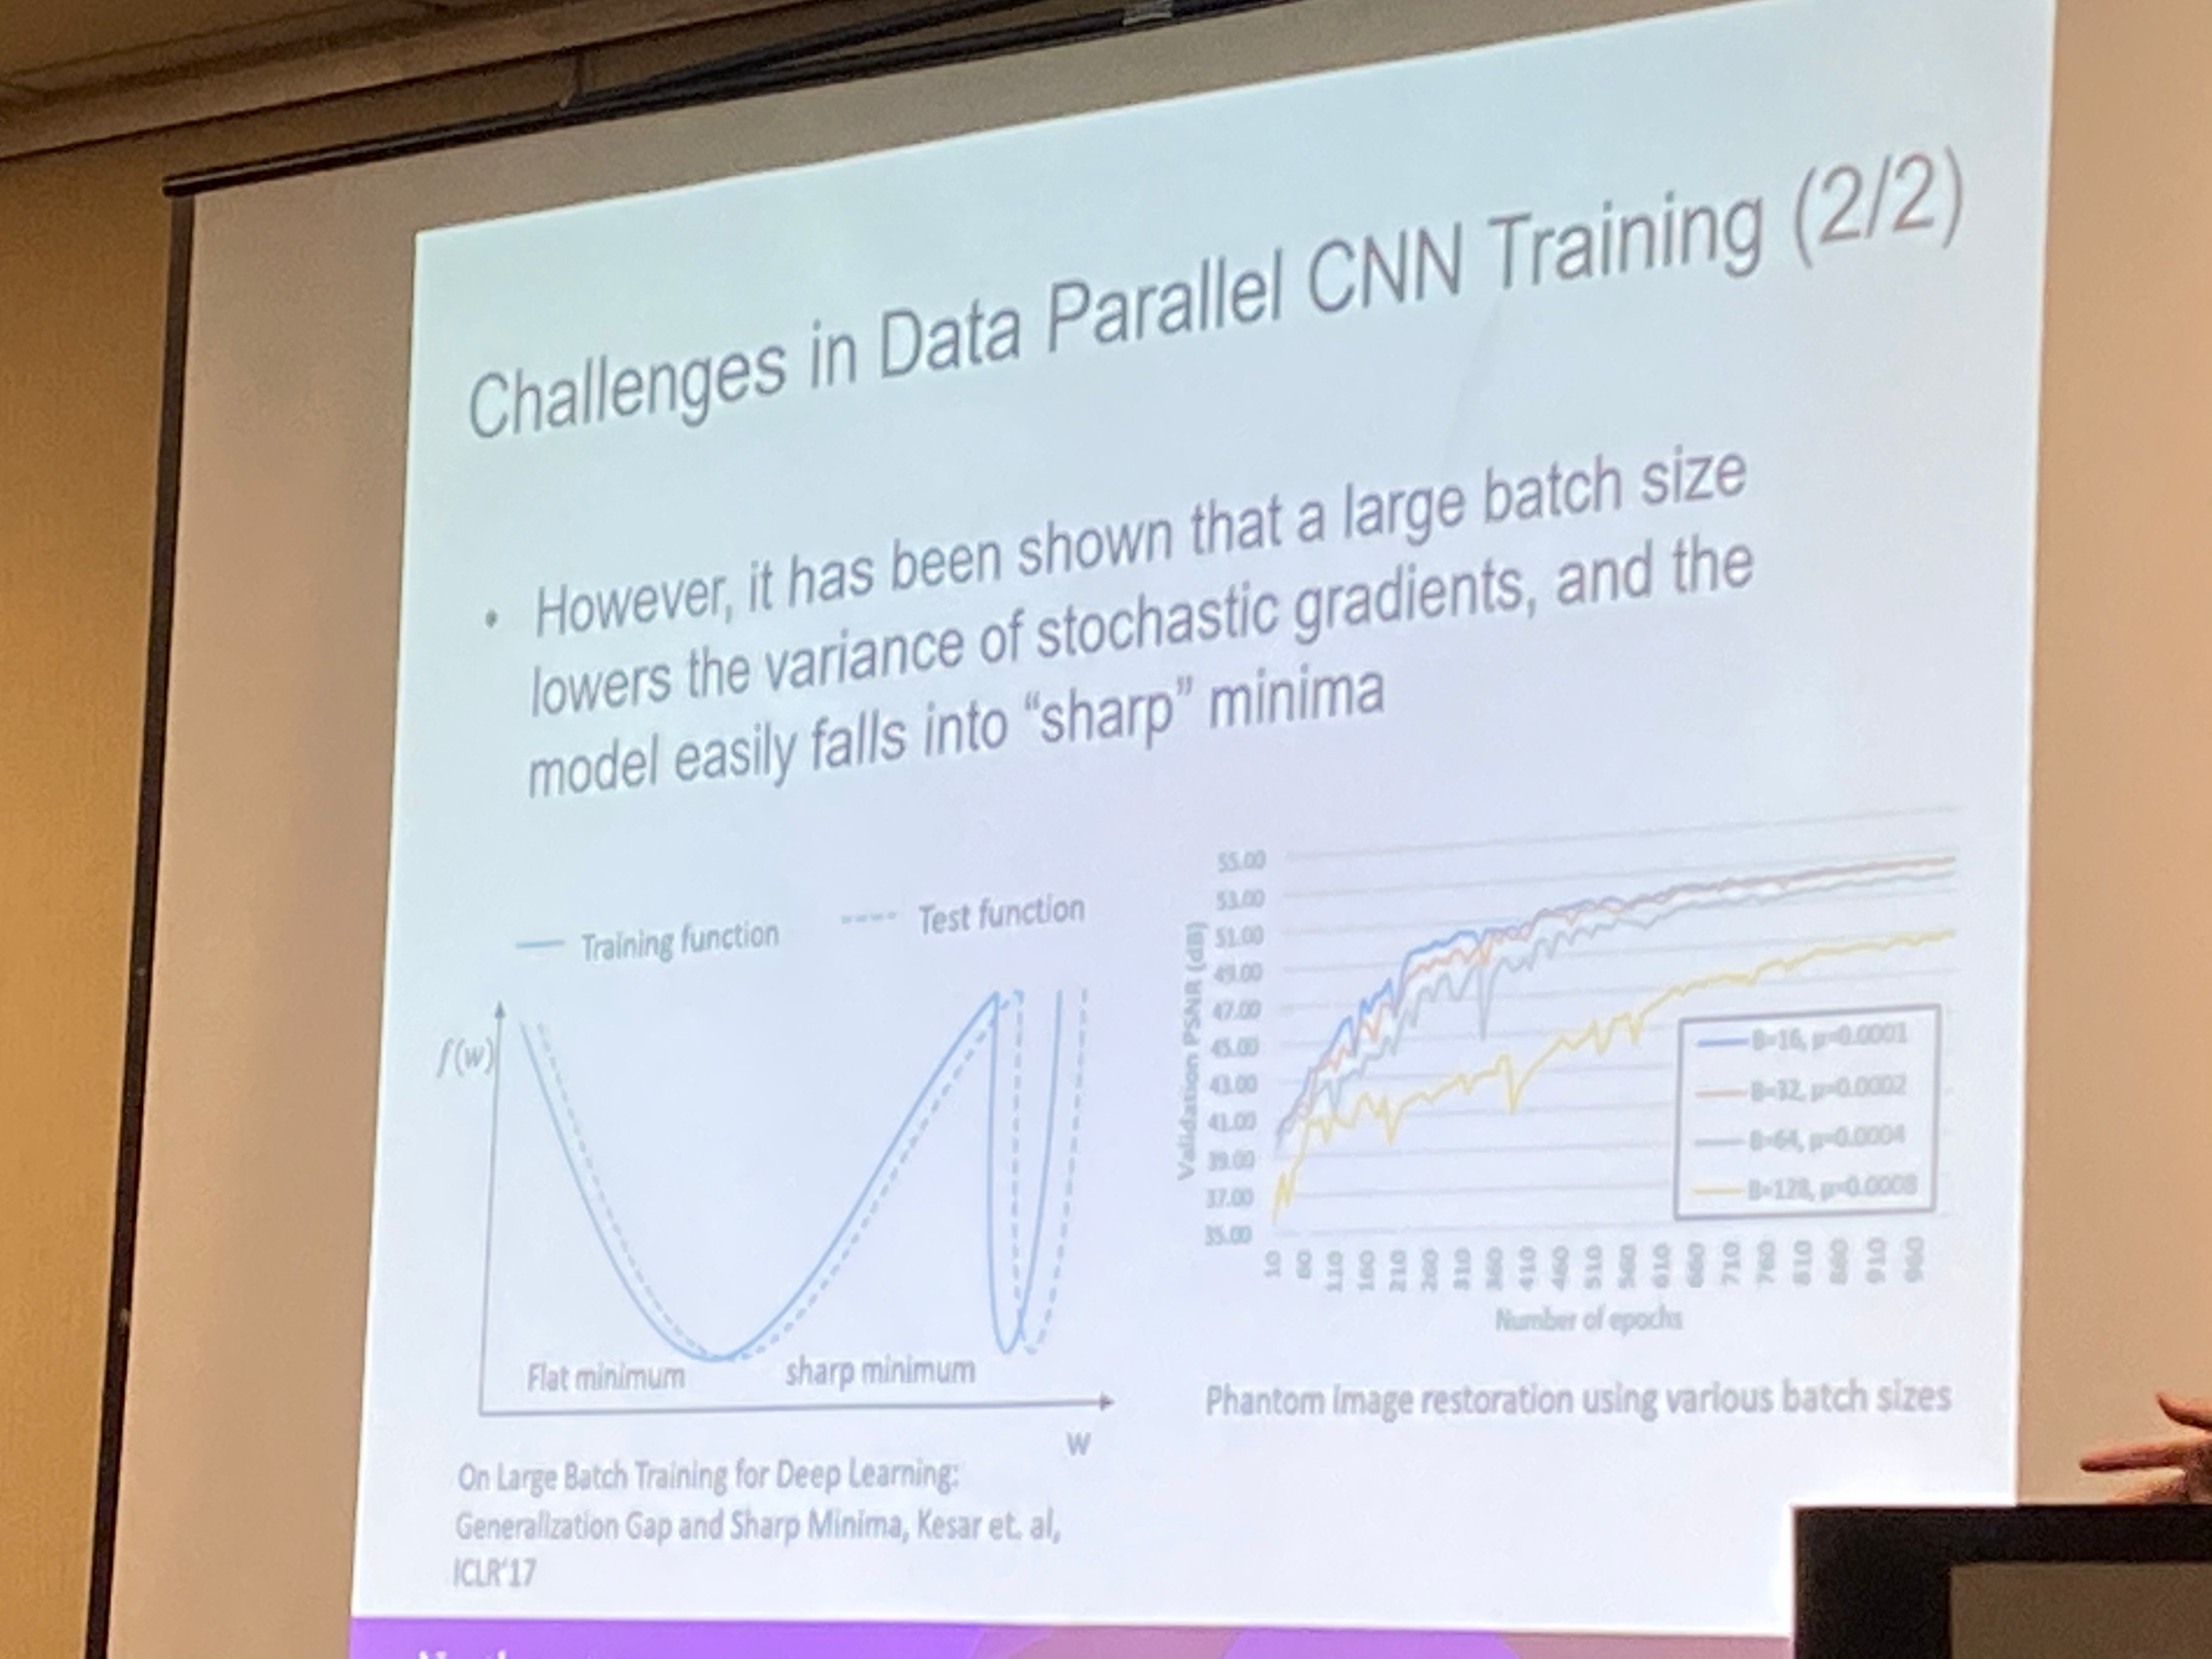
\includegraphics[width=120mm]{images/cnn_parallel_2.png}
    \caption{Data parallel CNN training2}
    \label{fig:my_label}
\end{figure}{}



\spacerule